% Канонический TikZ-рисунок варианта 33. Править только здесь.
\long\def\figStereoV33{%
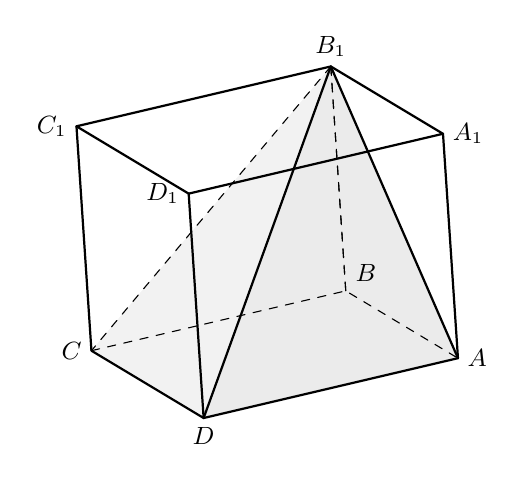
\begin{tikzpicture}[
  scale=0.95,
  line cap=round,
  line join=round,
  every node/.style={font=\small}
]
  % Нижнее основание параллелепипеда
  % Фигура специально развёрнута:
  % вершины B и D не лежат на одной вертикали
  \coordinate (A) at ( 2.7, 0.1);
  \coordinate (B) at ( 1.2, 1.0);
  \coordinate (C) at (-2.2, 0.2);
  \coordinate (D) at (-0.7,-0.7);

  % Верхнее основание
  \coordinate (A1) at ( 2.5,3.1);
  \coordinate (B1) at ( 1.0,4.0);
  \coordinate (C1) at (-2.4,3.2);
  \coordinate (D1) at (-0.9,2.3);

  % Полупрозрачные грани искомого многогранника ABCDB_1
  \fill[black!5]
    (B1)--(C)--(D)--cycle;

  \fill[black!8]
    (B1)--(D)--(A)--cycle;

  % Нижнее основание:
  % передние рёбра
  \draw[thick] (C)--(D)--(A);

  % задние рёбра
  \draw[dashed] (C)--(B)--(A);

  % Верхнее основание параллелепипеда
  \draw[thick]
    (C1)--(B1)--(A1)--(D1)--cycle;

  % Боковые рёбра параллелепипеда
  \draw[thick]  (C)--(C1);
  \draw[thick]  (D)--(D1);
  \draw[thick]  (A)--(A1);
  \draw[dashed] (B)--(B1);

  % Рёбра искомого многогранника
  \draw[dashed] (B1)--(C);
  \draw[thick] (B1)--(D);
  \draw[thick] (B1)--(A);

  % Скрытое ребро B_1B
  \draw[dashed] (B1)--(B);

  % Подписи нижнего основания
  \node[right]       at (A) {$A$};
  \node[above right] at (B) {$B$};
  \node[left]        at (C) {$C$};
  \node[below]       at (D) {$D$};

  % Подписи верхнего основания
  \node[right] at (A1) {$A_1$};
  \node[above] at (B1) {$B_1$};
  \node[left]  at (C1) {$C_1$};
  \node[left]  at (D1) {$D_1$};
\end{tikzpicture}
}
